\chapter{Image Based Profiling}

Modern fluorescence microscopy combined with high throughput biotechnology, automatically quantifying biological properties in images, is now widespread. They provides new insights into human cells and are powerful technologies for studying cell biology. 
Using this technology more than more than 
one hundred thousand  images can be produced per day.
This makes automated image analysis a necessity. 
Image-based profiling aims at getting as much data 
as possible from a biological sample and to encoding
it in a proper way. Image-based profiling experiments capture a wide range of data
from biological samples without prior knowledge
of the existence of any markers.
Data mining and machine learning techniques can then be applied to identify patterns \cite{Jones} \cite{Scheeder2018}.

\subsection{Drug discovery}

One important application of image-based profiling is identifying biological mechanisms of actions (MOA),
for example checking damage of DNA replications due to chemical perturbations.
When developing new drugs and making predictions about unknown
chemical compounds it is important to know what chemical compounds cause which biological mechanisms of action.
Morphological profiles can predict these MOAs for chemical compounds.

\subsection{Typical workflow}

There are two approaches in image-based phenotyping of perturbations. 
It should be considered that they are different.
The first approach is called phenotypic screening. 
Phenotypic screening uses pre-defined, specific phenotypes which are compared 
with the specimen in order to identify drugs or drug targets that might have affected 
them.

The second method is called profiling of perturbations. 
Here a computer is trained with a large set of samples, both
affected by perturbations and unaffected ones.
Once trained the computer can analyze new specimen 
and for perturbed ones identify the drugs or drug targets that have affected them.
This approach doesn't require the specification of any features such as cell size, intensity, shape, or texture.
It furthermore permits how any specimen would look if it was affected by a specific perturbation.


\begin{figure}[H]
	\centering
	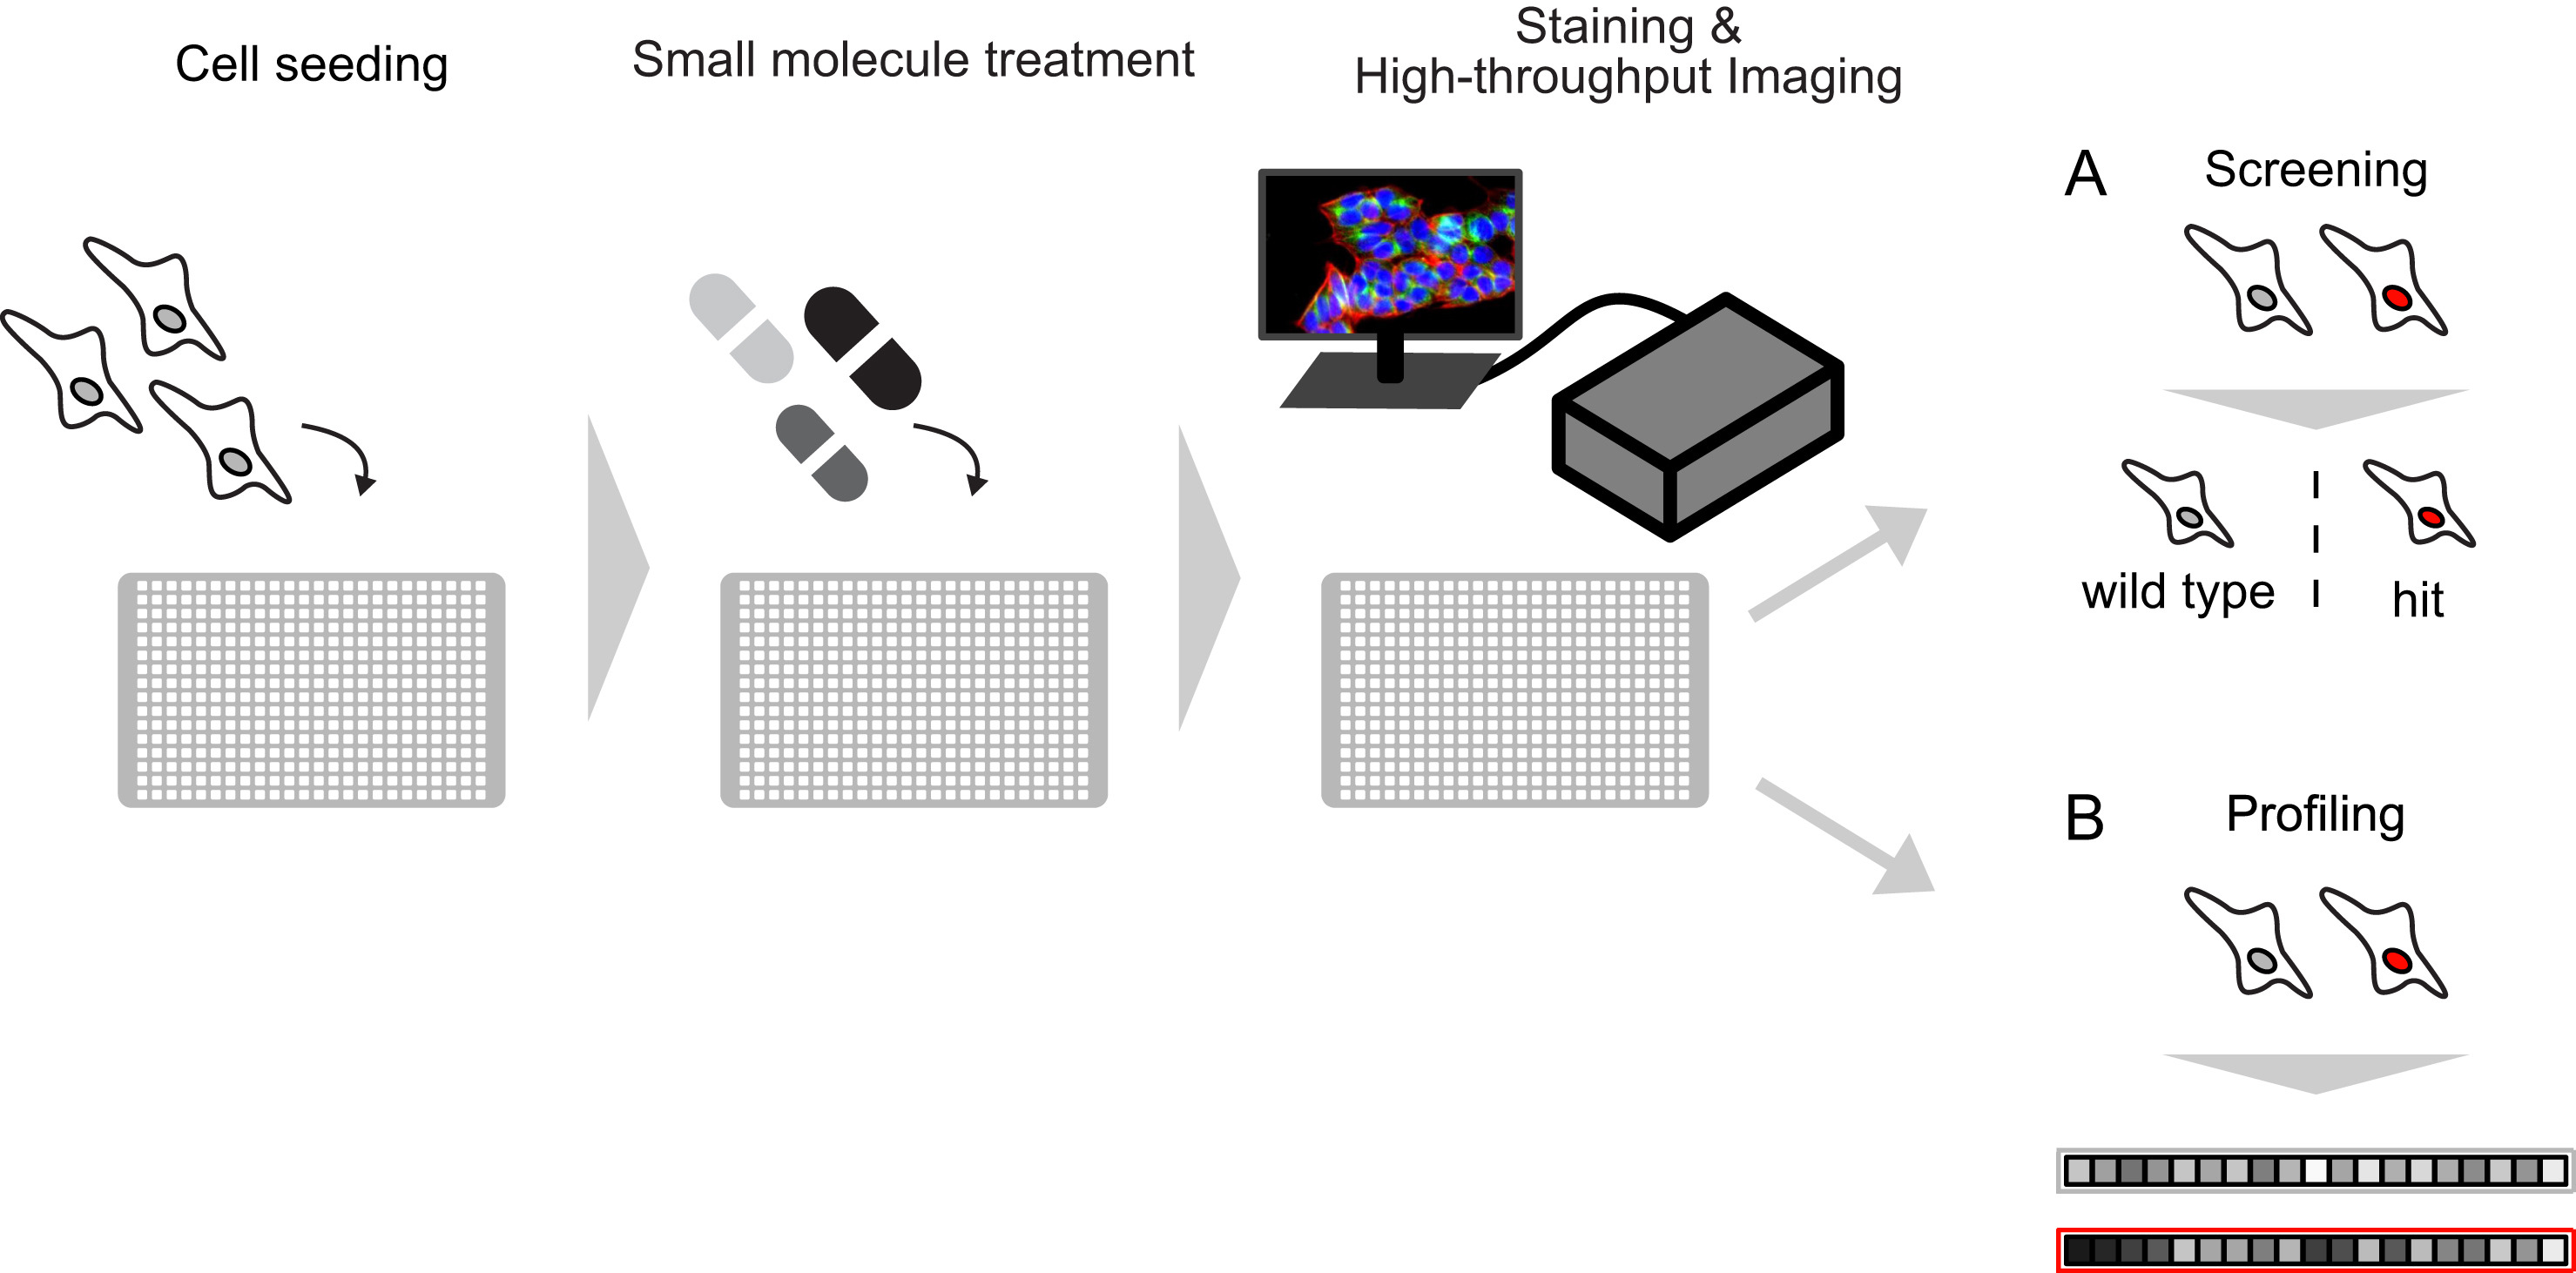
\includegraphics[width=0.8\linewidth]{bilder/cells/hcu.png}
	\caption{Typical workflow of image-based small molecule experiments (from\cite{Scheeder2018})}
	\label{fig:Workflow}
\end{figure}

Fig. \ref{fig:Workflow} illustrates a typical workflow of image-based small molecule experiments. First cells need to be attached to plates. In a second step cells are perturbed. Then after staining the cells, images are taken using automated microscopes. At the end either screening approaches (A) or (B) profiling approaches can be used to classify perturbed cells.

\subsubsection{Segmentation}

Small molecule profiling is based on staining subcellular structures (Fig. \ref{fig:ig:Segmentation}).
An accurate segmentation of cells can be achieved by in intensity-based thresholding and other approaches. A number of computational applications for segmentation-free analysis in image-based profiling have been developed, the most famous one being the Cell Profiler \cite{CellProfiler}.


\begin{figure}[H]
	\centering
	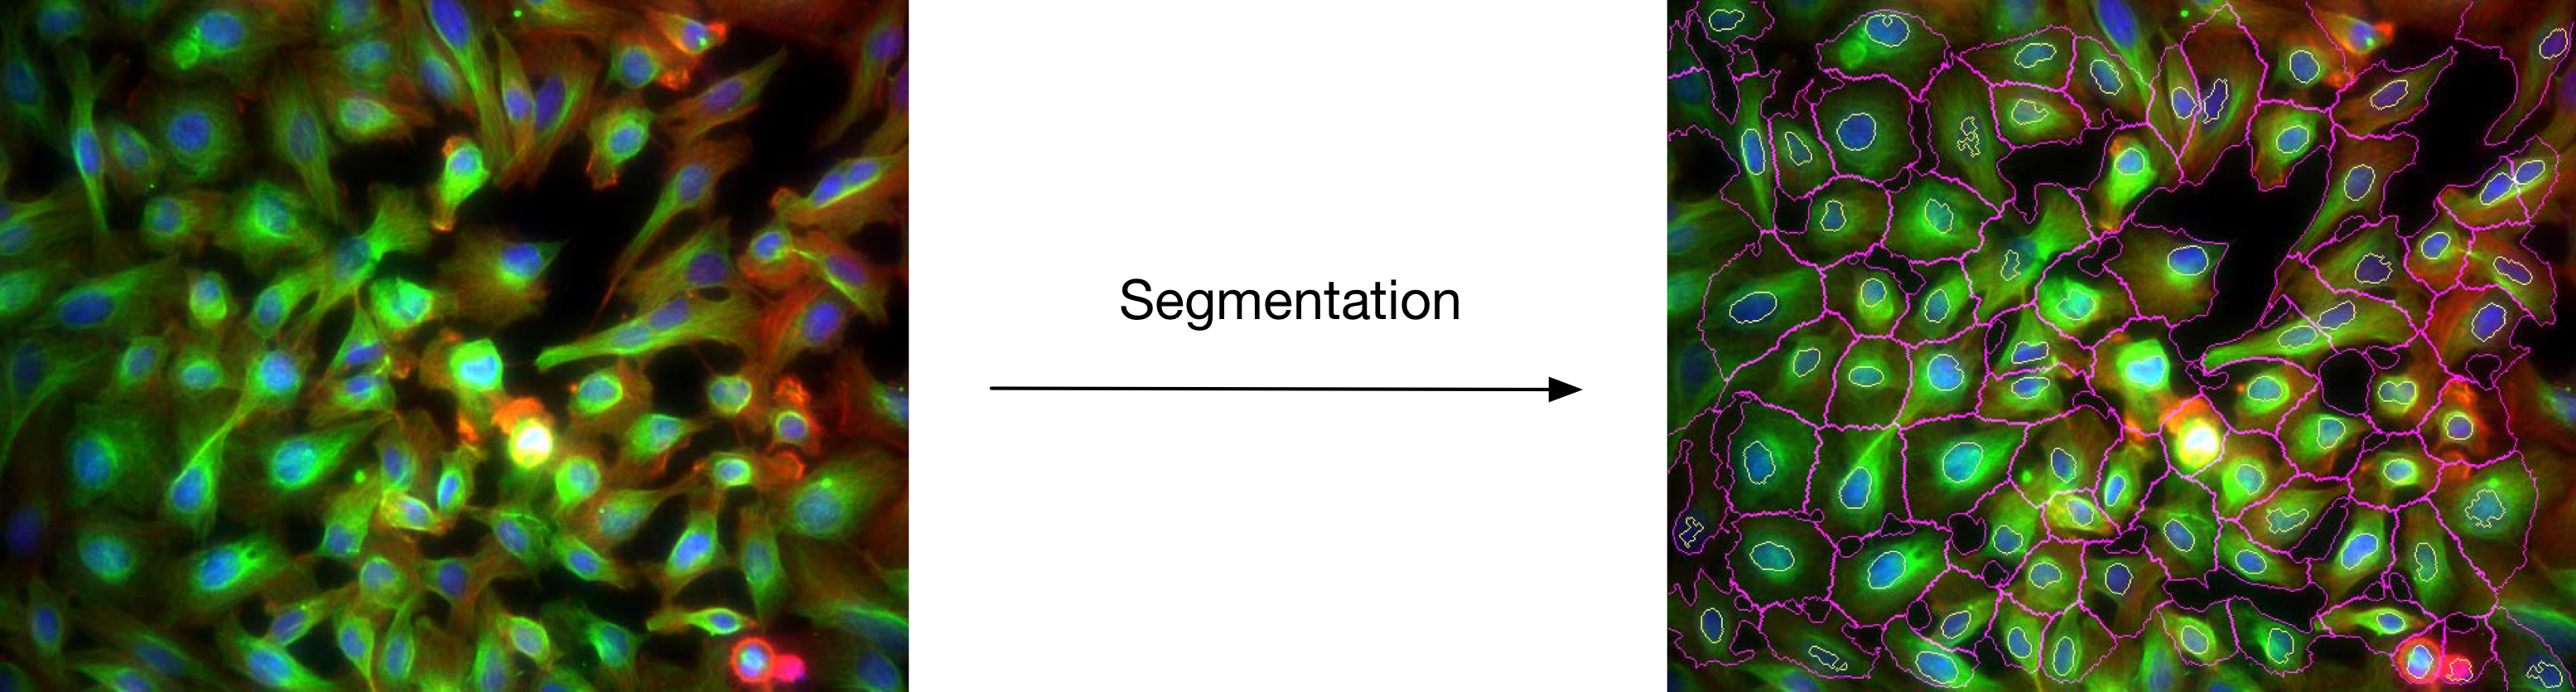
\includegraphics[width=0.8\linewidth]{bilder/cells/segmentation.png}
	\caption{Segmentation (from \cite{Pau})}
	\label{fig:Segmentation}
\end{figure}


\subsubsection{Classification}


A typical objective for profiling experiments is the classification of compounds that cells have been perturbed with. 
Common classifiers are random forests and deep neural networks that are employed to achieve higher 
accuracy in predicting biological MOAs.


\begin{figure}[H]
	\centering
	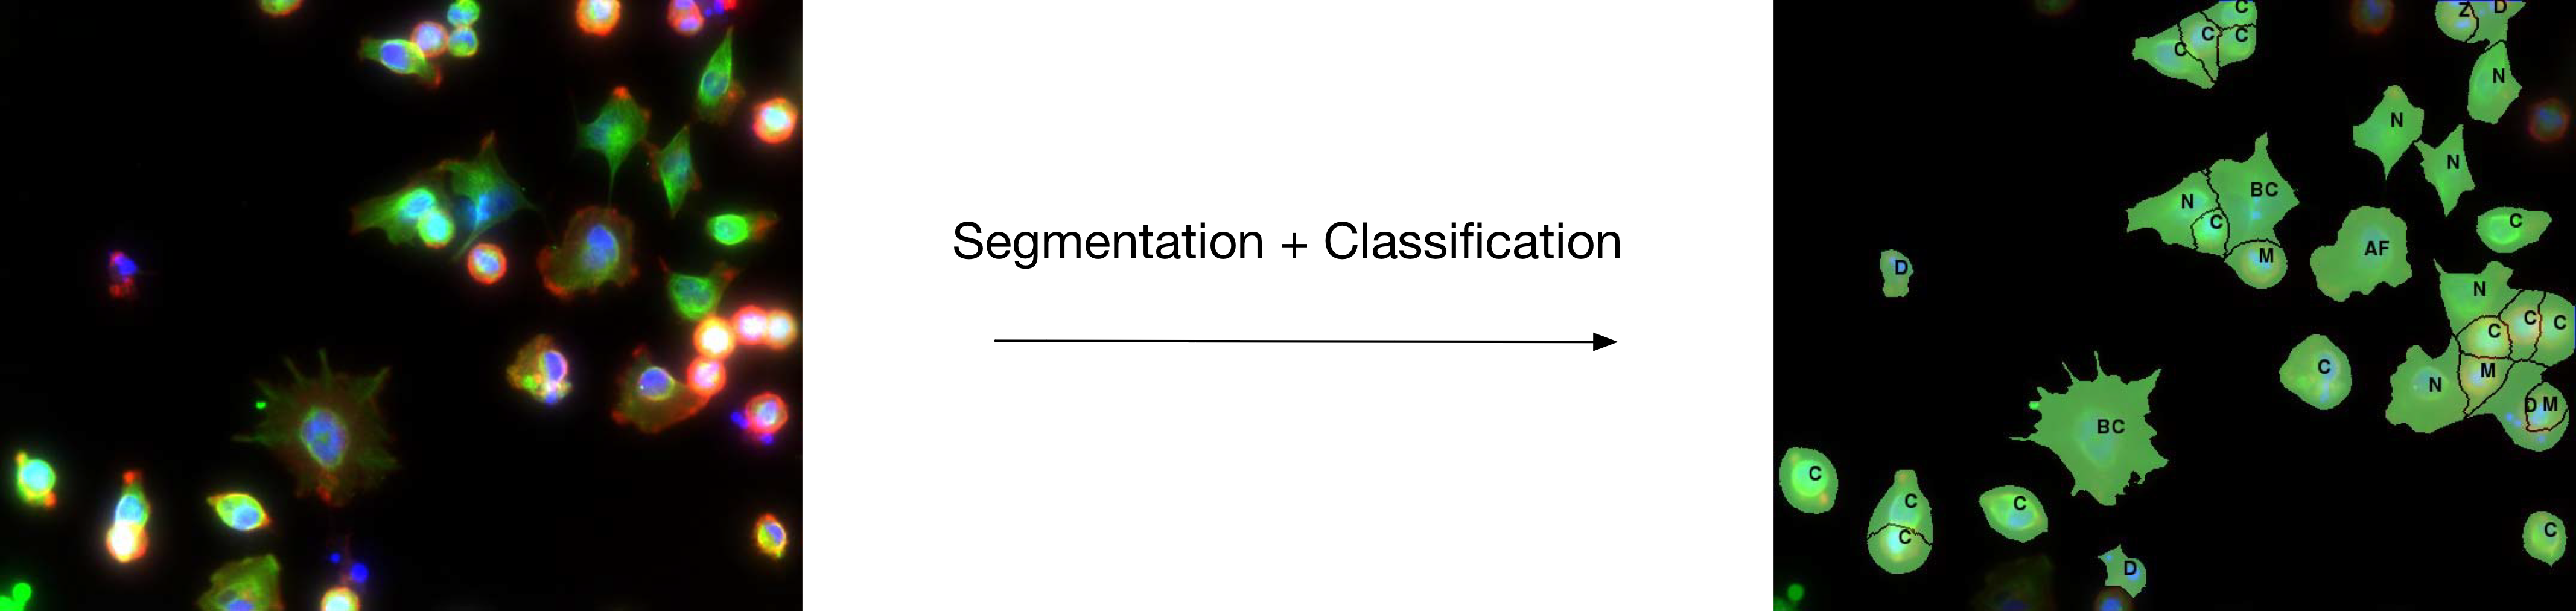
\includegraphics[width=0.8\linewidth]{bilder/cells/classification.png}
	\caption{Classification  (from \cite{Pau})}
	\label{fig:Classification}
\end{figure}




